\documentclass{beamer}
\usepackage{listings}
\usepackage{hyperref}
\usepackage{tikz}
\usetikzlibrary{positioning,shadows,arrows,shapes,calc}
\def\labelenumi\theenumi
\usepackage{graphicx}
\usepackage{amsmath}
\mode<presentation>{\usetheme{Frankfurt}}
\AtBeginSection
{
  \begin{frame}<beamer>
    \frametitle{Outline}
    \tableofcontents[currentsection,currentsubsection]
  \end{frame}
}
\title{Lecture 22: Variational Autoencoder\\Reference: \href{https://arxiv.org/pdf/1312.6114.pdf}{Kingma \& Welling (2013)}}
\author{Mark Hasegawa-Johnson\\All content~\href{https://creativecommons.org/licenses/by-sa/4.0/}{CC-SA 4.0} unless otherwise specified.}
\date{ECE 417: Multimedia Signal Processing, Fall 2020}  
\institute{University of Illinois}
\titlegraphic{\includegraphics{../../../17fall/lectures/imark_1867_bold.png}}
\begin{document}

% Title
\begin{frame}
  \maketitle
\end{frame}

% Title
\begin{frame}
  \tableofcontents
\end{frame}

%%%%%%%%%%%%%%%%%%%%%%%%%%%%%%%%%%%%%%%%%%%%%%%%%%%%%%%%%
\section{Autoencoders}
\setcounter{subsection}{1}

\begin{frame}
  \frametitle{Autoencoder}

  An {\bf autoencoder} is a neural net that learns a hidden code,
  $\vec{h}$, that is sufficient to reconstruct $\vec{x}$:
  \begin{align*}
    \vec{h} &= f(\vec{x})\\
    \hat{x} &= g(\vec{h})
  \end{align*}
  An autoencoder is usually trained to minimize mean-squared error,
  equivalent to maximizing the likelihood of a spherical Gaussian
  model:
  \begin{displaymath}
    {\mathcal L}=\sum_{i=1}^n \Vert\hat{x}_i-\vec{x}_i\Vert^2
  \end{displaymath}
\end{frame}

\begin{frame}
  \frametitle{Autoencoder}

  \centerline{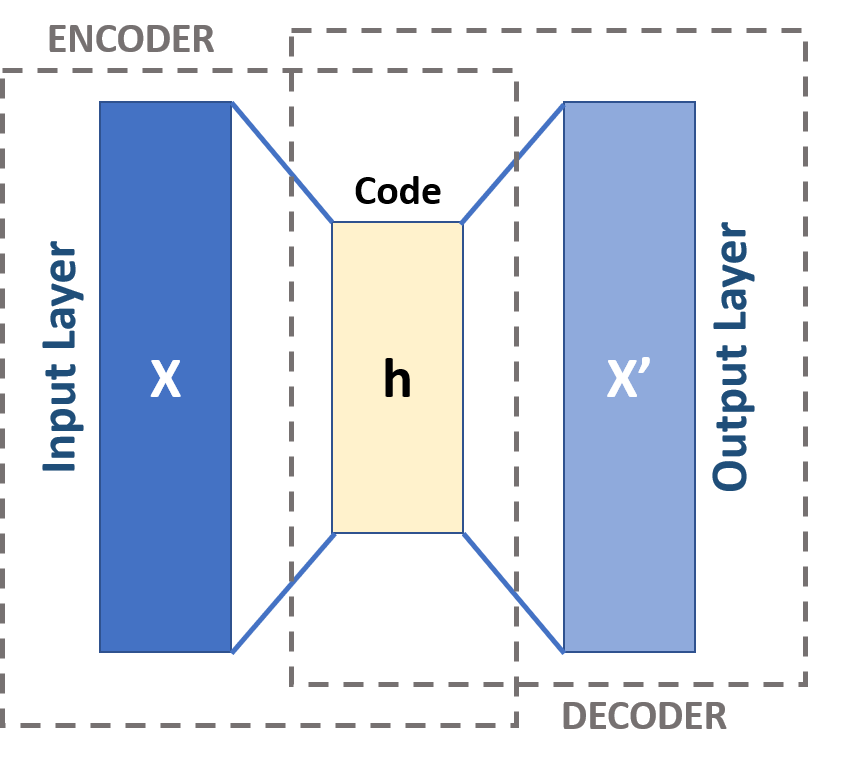
\includegraphics[height=2in]{Autoencoder_schema.png}}
  \begin{tiny}
    Image Michela Massi, 2019, CC-SA 4.0,
    \url{https://commons.wikimedia.org/wiki/File:Autoencoder_schema.png}
  \end{tiny}
\end{frame}

\begin{frame}
  \frametitle{Linear Two-layer Autoencoder = PCA}

  Consider a two-layer linear autoencoder:
  \begin{align*}
    \vec{h} &= W^T(\vec{x}-\vec{b})\\
    \hat{x} &= W\vec{h}+\vec{b}
  \end{align*}
  The loss becomes
  \begin{displaymath}
    {\mathcal L}=\sum_{i=1}^n \Vert\vec{x}_i-WW^T(\vec{x}-\vec{b})-\vec{b}\Vert^2
  \end{displaymath}
\end{frame}

\begin{frame}
  \frametitle{Linear Two-layer Autoencoder = PCA}
  \begin{displaymath}
    {\mathcal L}=\sum_{i=1}^n \Vert\vec{x}_i-WW^T(\vec{x}-\vec{b})-\vec{b}\Vert^2
  \end{displaymath}
  \begin{itemize}
  \item If $\mbox{len}(\vec{h})\ge\mbox{len}(\vec{x})$, then the
    optimum solution is $W=I$, $\vec{b}=\vec{0}$, and $\hat{x}=\vec{x}$.
  \item If $\mbox{len}(\vec{h})<\mbox{len}(\vec{x})$, then PCA minimizes ${\mathcal L}$.
    \begin{itemize}
    \item $\vec{b}=$ the data mean,
    \item $W=$ the matrix of principal component directions.
    \end{itemize}
  \end{itemize}
\end{frame}

\begin{frame}
  \frametitle{Types of Autoencoders}

  If the hidden layer has too few constraints, we can get perfect
  reconstruction without learning anything useful.  In order to learn
  useful hidden representations, a few common constraints are:
  \begin{itemize}
  \item Low-dimensional hidden layer.  In this case, $\vec{h}$ is a
    nonlinear generalization of PCA, sometimes called a {\bf bottleneck.}
  \item {\bf Sparse autoencoder}: use a large hidden layer, but
    regularize the loss using a penalty that encourages $\vec{h}$ to
    be mostly zeros, e.g.,
    \begin{displaymath}
      {\mathcal L}=\sum_{i=1}^n \Vert\hat{x}_i-\vec{x}_i\Vert^2 + \lambda\sum_{i=1}^n\Vert\vec{h}_i\Vert_1
    \end{displaymath}
  \item {\bf Variational autoencoder:} like a sparse autoencoder, but
    the penalty encourages $\vec{h}$ to match a predefined prior distribution,
    $p_\theta(\vec{h})$.
  \end{itemize}
\end{frame}

%%%%%%%%%%%%%%%%%%%%%%%%%%%%%%%%%%%%%%%%%%%%%%%%%%%%%%%%%
\section{Variational Bayes}
\setcounter{subsection}{1}

\begin{frame}
  \frametitle{Bayesian Learning}

  The goal of Bayesian learning is to learn a complete model of the
  probability density function, $p(\vec{x})$.  We usually assume that
  there is some latent variable $\vec{z}$, and a set of parameters
  $\theta$, such that
  \begin{itemize}
  \item $\vec{z}$ is a latent variable generated randomly according to
    $p_\theta(\vec{z})$
  \item $\vec{x}$ is then generated randomly according to
    $p_\theta(\vec{x}|\vec{z})$
  \end{itemize}
\end{frame}

\begin{frame}
  \frametitle{Bayesian Learning}

  A hidden Markov model is an example of Bayesian learning. We can
  generalize the three problems of an HMM, using the words of (Kingma
  and Welling, 2013):
  \begin{enumerate}
  \item {\bf Recognition:} Efficient approximate
    marginal inference of the variable $\vec{x}$.  Besides comparing
    different models, this can also allow us to generate synthetic
    data using $p_\theta(\vec{x})$.
  \item {\bf Segmentation:} Efficient approximate posterior inference
    of the latent variable $\vec{z}$ given an observed value $\vec{x}$
    for a choice of parameters $\vec\theta$.
  \item {\bf Learning:} Efficient approximate ML or MAP estimation for
    the parameters $\vec\theta$.
  \end{enumerate}
\end{frame}

\begin{frame}
  \frametitle{Variational Bayes: Intractable Posteriors}

  \begin{itemize}
  \item Variational Bayes is used in cases like the HMM, when
    \begin{itemize}
      \item the {\bf likelihood}, $p_\theta(\vec{x}|\vec{z})$, is easy to compute,
        but
      \item the {\bf posterior}, $p_\theta(\vec{z}|\vec{x})$, is intractable.
    \end{itemize}
  \item If $p_\theta(\vec{z}|\vec{x})$ is intractable, then we can't
    exactly solve the segmentation or learning problems.  Instead, we
    introduce a {\bf variational approximation},
    $q_\phi(\vec{z}|\vec{x})\approx p_\theta(\vec{z}|\vec{x})$, and
    try to learn parameters $\phi$ and $\theta$
    in order to match the data as well as possible.
  \end{itemize}
\end{frame}

\begin{frame}
  \frametitle{The Evidence Lower Bound}

  Variational Bayes learns parameters $\theta$ and $\phi$ in order to
  maximize the {\bf evidence} distribution:
  \begin{displaymath}
    \ln p_\theta(\vec{x})
  \end{displaymath}
  \begin{itemize}
  \item Averaging over the training data is understood.
  \end{itemize}
\end{frame}

\begin{frame}
  \frametitle{The Evidence Lower Bound}

  Since the evidence doesn't depend on $\vec{z}$ at all, it doesn't
  hurt to compute its expected value w.r.t. $\vec{z}$:
  \begin{align*}
    \ln p_\theta(\vec{x})
    &=E_{q_\phi(\vec{z}|\vec{x})}\left[\ln p_\theta(\vec{x})\right]
  \end{align*}
\end{frame}

\begin{frame}
  \frametitle{The Evidence Lower Bound}

  We can introduce $\vec{z}$ inside the expectation by using the
  definition of conditional probability,
  $p(\vec{x},\vec{z})=p(\vec{x})p(\vec{z}|\vec{x})$, to get:
  \begin{align*}
    \ln p_\theta(\vec{x})
    &=E_{q_\phi(\vec{z}|\vec{x})}
    \left[
      \ln\left(
      \frac{p_\theta(\vec{x},\vec{z})}{p_\theta(\vec{z}|\vec{x})}
      \right)
      \right]
  \end{align*}
\end{frame}

\begin{frame}
  \frametitle{The Evidence Lower Bound}

  Now, we can introduce $q_\phi$ inside the expectation as:
  \begin{align*}
    \ln p_\theta(\vec{x})
    &=E_{q_\phi(\vec{z}|\vec{x})}
    \left[
      \ln\left(
      \frac{p_\theta(\vec{x},\vec{z})}{p_\theta(\vec{z}|\vec{x})}
      \frac{q_\phi(\vec{z}|\vec{x})}{q_\phi(\vec{z}|\vec{x})}
      \right)
      \right]
  \end{align*}
\end{frame}

\begin{frame}
  \frametitle{Kullback-Leibler Divergence}

  Claude Shannon introduced a measure of the difference between two
  probability densities, called the Kullback-Leibler divergence:
  \begin{displaymath}
    D_{KL}\left(q_\phi(\vec{z}|\vec{x})\Vert p_\theta(\vec{z}\Vert\vec{x})\right)
    =
    E_{q(\vec{z}|\vec{x})}
    \left[
      \ln\left(\frac{q_\phi(\vec{z}|\vec{x})}{p_\theta(\vec{z}|\vec{x})}\right)
      \right]
  \end{displaymath}
  A useful thing to know about KLD is that it's always non-negative:
  $D_{KL}(q\Vert p)\ge 0$, with equality if and only if $q=p$.
\end{frame}

\begin{frame}
  \frametitle{The Evidence Lower Bound}

  Re-arranging terms inside the expectation, we get
  \begin{align*}
    \ln p_\theta(\vec{x})
    &=
    D_{KL}\left(q_\phi(\vec{z}|\vec{x})\Vert p_\theta(\vec{z}|\vec{x})\right)
    + {\mathcal L}\left(\theta,\phi;\vec{x}\right)
  \end{align*}
  and therefore
  \begin{align*}
    \ln p_\theta(\vec{x}) &\ge {\mathcal L}\left(\theta,\phi;\vec{x}\right)
  \end{align*}
  with equality if and only if
  $q_\phi(\vec{z}|\vec{x})=p_\theta(\vec{z}|\vec{x})$.  The term
  ${\mathcal L}\left(\theta,\phi;\vec{x}\right)$ is therefore called the
  evidence lower bound or ELBO, and is given by
  \begin{displaymath}
    {\mathcal L}\left(\theta,\phi;\vec{x}\right) =
    E_{q(\vec{z}|\vec{x})}\left[\ln p_\theta(\vec{x},\vec{z})-\ln q_\phi(\vec{z}|\vec{x})\right]
  \end{displaymath}
\end{frame}

\begin{frame}
  \frametitle{Summary: Variational Bayes}

  \begin{itemize}
  \item Variational Bayes is a method for learning a latent-variable
    model that can be used to generate synthetic data, encode the
    data, or recognize the data.
  \item It solves the intractability of $p_\theta(\vec{z}|\vec{x})$ by
    introducing a variational approximation,
    $q_\phi(\vec{z}|\vec{x})\approx p_\theta(\vec{z}|\vec{x})$.
  \item The intractable term $p_\theta(\vec{z}|\vec{x})$ is then
    eliminated from the evidence by wrapping it up inside
    $D_{KL}\left(q_\phi(\vec{z}|\vec{x})\Vert
    p_\theta(\vec{z}\Vert\vec{x})\right)$.  Since KLD is always
    non-negative, we can eliminate it from training criterion, leaving
    us with the evidence lower bound:
    \begin{displaymath}
      {\mathcal L}\left(\theta,\phi;\vec{x}\right) =
      E_{q(\vec{z}|\vec{x})}\left[\ln p_\theta(\vec{x},\vec{z})-\ln q_\phi(\vec{z}|\vec{x})\right]
    \end{displaymath}
  \end{itemize}
\end{frame}




%%%%%%%%%%%%%%%%%%%%%%%%%%%%%%%%%%%%%%%%%%%%%%%%%%%%%%%%%
\section{Variational Autoencoder}
\setcounter{subsection}{1}

\begin{frame}
  \frametitle{The Problem with Variational Bayes}

  All previous VB algorithms struggled with the problem of efficiently
  computing expectations of the form
  $E_{q(\vec{z}|\vec{x})}\left[f(\vec{z})\right]$.
  Two tricks were commonly used, each with its own  problems:
  \begin{itemize}
  \item {\bf Factoring:} assume that $q(\vec{z}|\vec{x})$ has some
    simple form, e.g., assume that the dimensions of $\vec{z}$ are
    independent given $\vec{x}$.  Problem: sometimes, no reasonable
    simplification of this type is possible.
  \item {\bf Sampling (Monte Carlo methods):} draw $L$ samples
    $\vec{z}^{(l)}$ from the distribution $q(\vec{z}|\vec{x})$, and
    then approximate
    \begin{displaymath}
      E_{q(\vec{z}|\vec{x})}\left[f(\vec{z})\right]\approx
      \frac{1}{L}\sum_{l=1}^L f(\vec{z}^{(l)})
    \end{displaymath}
    Problem: if $q(\vec{z}|\vec{x})$ is a complicated distribution
    with many local maxima, then the approximation may be very bad,
    even for relatively large values of $L$.
  \end{itemize}
\end{frame}

\begin{frame}
  \frametitle{Kingma \& Welling: The Reparameterization Trick}

  Kingma \& Welling (2013) proposed a reparameterization trick: assume
  \begin{displaymath}
    \vec{z}^{(l)}=g_\phi(\vec\epsilon^{(l)},\vec{x}),
  \end{displaymath}
  where $g_\phi$ is a flexible universal approximator (a neural net),
  and $\vec\epsilon$ is drawn from a predefined unimodal compact
  probability density function, e.g., a unit-normal Gaussian or
  uniform distribution.  The sample average of a Gaussian or uniform
  distribution approaches its true average very quickly, e.g., even
  for $L\approx 5J$, where $J=\mbox{len}(\vec{z})$. Kingma \& Welling
  recommend using a minibatch of about 100 training tokens, with $L=1$
  for each training token.
  \begin{displaymath}
    E_{q(\vec{z}|\vec{x})}\left[f(\vec{z})\right]\approx
    \frac{1}{L}\sum_{l=1}^L f(g_\phi(\vec\epsilon^{(l)},\vec{x}))
  \end{displaymath}
\end{frame}

\begin{frame}
  \frametitle{Kingma \& Welling: The Reparameterization Trick}

  The reparameterization trick is most useful if you assume that the
  latent variable has a parameter-independent prior, e.g.,
  $p_\theta(\vec{z})=p(\vec{z})={\mathcal N}(\vec{0},I)$.  Then you
  can re-write the ELBO as
  \begin{align*}
    {\mathcal L}\left(\theta,\phi;\vec{x}\right) &=
    -D_{KL}\left(q_\phi(\vec{z}|\vec{x})\Vert p_\theta(\vec{z})\right) +
    E_{q(\vec{z}|\vec{x})}\left[\ln p_\theta(\vec{x}|\vec{z})\right]\\
    &\approx 
    -D_{KL}\left(q_\phi(\vec{z}|\vec{x})\Vert p(\vec{z})\right) +
    \frac{1}{L}\sum_{l=1}^L\ln p_\theta(\vec{x}|\vec{z}^{(l)})
  \end{align*}
  \begin{itemize}
  \item The second term, $\ln p_\theta(\vec{x}|\vec{z}^{(l)})$, is a
    neural network parameterized by $\theta$.
  \item The first term, $-D_{KL}\left(q_\phi(\vec{z}|\vec{x})\Vert
    p(\vec{z})\right)$, needs to be solved by pencil and paper.
  \end{itemize}
\end{frame}

\begin{frame}
  \frametitle{Variational Autoencoder}

  The variational autoencoder has the following steps.
  For each training token,
  \begin{enumerate}
  \item Use a neural network, parameterized by $\phi$, to compute the
    posterior mean and variance of the latent variable:
    \begin{displaymath}
      q_\phi(\vec{z}|\vec{x})=
      {\mathcal N}\left(\vec\mu_{\vec{z}}(\vec{x};\phi),\Sigma_{\vec{z}}(\vec{x};\phi)\right)
    \end{displaymath}
    where ${\mathcal N}(\vec\mu,\Sigma)$ is the normal distribution,
    $\vec\mu_{\vec{z}}(\vec{x};\phi)$ and
    $\Sigma_{\vec{z}}(\vec{x};\phi)$ are the mean and variance
    of $\vec{z}$ conditioned on $\vec{x}$ and $\phi$.
  \item Draw $L$ random $\vec{z}$ vectors from the distribution (e.g.,
    $L=1$).
  \item Estimate $p_\theta(\vec{x}|\vec{z})$ using another neural network,
    parameterized by $\theta$.
  \item Update $\theta$ and  $\phi$ using gradient ascent.
  \end{enumerate}
\end{frame}

\begin{frame}
  \frametitle{Benefits and Drawbacks of VAE}

  \begin{itemize}
  \item A key benefit of the VAE is interpretability.  You have two
    networks: one that generates $\vec{z}$ from $\vec{x}$, and one
    that generates $\vec{x}$ from $\vec{z}$.  Therefore, you can map
    out the latent space, observing what types of data vectors
    $\vec{x}$ are generated from each point in the latent space.
  \item Another key benefit is generation.  The latent variable is
    forced to have the distribution ${\mathcal N}(\vec{0},I)$, so it's
    easy to generate synthetic data.
  \item A drawback is over-smoothing.  VAE is trained to maximize the
    evidence of the training data, i.e., the likelihood marginalized
    over all latent variables.  Maximum-likelihood models tend to
    generate synthetic data that is over-smoothed, more like an
    average of many images, instead of any particular image.
  \end{itemize}
\end{frame}

%%%%%%%%%%%%%%%%%%%%%%%%%%%%%%%%%%%%%%%%%%%%%%%%%%%%%%%%%
\section{Summary}
\setcounter{subsection}{1}
    
\begin{frame}
  \frametitle{Summary}

  \begin{itemize}
  \item Autoencoders try to find a latent vector that encodes as much
    information as possible about $\vec{x}$, subject to some
    constraints.
  \item Bayesian learning methods try to find a latent vector that
    encodes the data, subject to a known model of the prior and
    likelihood distributions.
  \item Variational Bayes avoids the intractability of the Bayesian
    posterior by using, instead, a variational approximation,
    $q_\phi(\vec{z}|\vec{x})\approx p_\theta(\vec{z}|\vec{x})$.  The
    difference between $q$ and $p$ is captured by their KLD, which is
    known to be non-negative, therefore VB can just maximize the
    ELBO.
  \item VAE models $q_\phi$ and $p_\theta$ using neural networks.  The
    ELBO then has two terms: reconstruction error (parameterized by
    $\theta$), and KLD between $q_\phi$ and a desired latent prior.
  \end{itemize}
\end{frame}

        
\end{document}

